\documentclass[11pt,a4paper]{ltxdoc} 
\usepackage[spanish,es-noindentfirst,es-tabla]{babel}

\usepackage[utf8]{inputenc}
\usepackage[T1]{fontenc}
\usepackage{graphicx}
\usepackage{mathpazo}
\usepackage{float}
\usepackage[margin=2.5cm,left=3.5cm]{geometry}
\usepackage{changelog}

\setlength{\parskip}{0.2\baselineskip}
\renewcommand{\baselinestretch}{1.1}

\newcommand{\file}[1]{\texttt{#1}}
\newcommand{\option}[1]{\texttt{#1}}
\newcommand{\package}[1]{\texttt{#1}}

\title{\file{aleph-libro.cls}}
\author{Proyecto Alephsub0\\ Andr\'es Merino\footnote{Escuela de Ciencias Físicas y Matemáticas, Pontificia Universidad Católica del Ecuador} \\ Daniel Lara\footnote{Facultad de Ciencias, Escuela Politécnica Nacional}}
\date{2023-12-24\\ Versión 2.0}

\begin{document}
 
\maketitle
 
\begin{abstract}
    \file{aleph-libro.cls} es una clase creada para dar formato a los libros y fascículos de libros con alto contenido matemático. Esta clase genera la portada de los libros, la contraportada, los ambientes utilizados, entre otros. Esta clase fue generada dentro del proyecto Alephsub0 (\url{https://www.alephsub0.org/}).
\end{abstract}

\section{Introducción}

La clase \file{aleph-libro.cls} es parte del conjunto de clases y paquetes creados por Andrés Merino dentro de su proyecto personal Alephsub0. Está basada en la clase \file{pubciencias-libro.cls} la cual, a su vez, se basa en la clase \file{PubCiencias.cls} (ambas del mismo autor) que recoge el formato de los primeros libros editados en la Unidad de Publicaciones de la EPN. Se actualizó el nombre de esta clase para continuar con el mantenimiento de la misma dentro del proyecto Alephsub0.
    
La clase provee el formato de la portada, portadilla, hoja de créditos,   contraportada, encabezados y pie de página, además del tamaño de página y márgenes de cada tipo de libro, los cuales se especifican como opción de la clase.

\section{Uso}

Para cargar la clase se utiliza: \cs{documentclass}\oarg{opciones}|{aleph-libro}| con las opciones acordes al formato que se desee.

\subsection{Opciones}

Las opciones de la clase son las siguientes:
\begin{description}
    \item[|10pt|, |11pt|, |12pt|] ajustan el tamaño de fuente. Por defecto, se usa |10pt|.
    \item[|amplio|, |compacto|] genera la geometría del libro predeterminada, es decir, tamaño de página y márgenes. Las dimensiones generadas por por estas opciones están dadas en la Tabla~\ref{tab:01}. Por defecto, se usa |compacto|.
    \item[|notasm|] aumenta el margen externo a 5cm y define las dimensiones necesarias para colocar notas al margen. Por defecto, esta opción está desactivada.
    \item[|numobs|] numera el ambiente de Observaciones predefinidas por la clase. Por defecto, esta opción está desactivada.
    \item[|npblanco|] elimina las páginas en blanco generadas luego de la portada y antes de la contraportada.
    \item[|fuente|] define la fuente que se utilizará en el documento. Las opciones disponibles son |mathpazo| y |montserrat|. Por defecto, se utiliza |mathpazo|.
\end{description}
  
\begin{table}[ht]
    \centering
    \begin{tabular}{cccccc}\hline
        Opción & Dimensiones & Interno & Externo & Superior & Inferior \\\hline
        |amplio| & 195mm$\times$265mm & 2.2cm & 2.5cm & 2.25cm & 2.25cm\\
        |compacto| & 160mm$\times$240mm & 2.2cm & 1.7cm & 2.25cm & 2.25cm\\
        \hline
    \end{tabular}
    \caption{Geometría de página predefinida.}
    \label{tab:01}
\end{table}

\subsection{Colores}

Las clase trabaja con dos colores básicos:
\begin{description}
    \item[|colorportada|] es el color de la portada y de los título.  El color predefinido por la clase es $(0.81,0.62,0.00,0.22)$ del formato |cmyk|.
    \item[|colordef|] es el color preestablecido para los ambientes de teoremas y notas al margen.  El color predefinido por la clase es $(0.81,0.62,0.00,0.22)$ del formato |cmyk|.
    \item[|colortext|] es el color preestablecido para los títulos $(0.81,0.62,0.00,0.22)$ del formato |cmyk|.
\end{description}
Se puede cambiar fácilmente estos colores con los comandos\\
    \hspace*{3em}\cs{definecolor}|{colorportada}|\marg{formato de color}\marg{color}\\
    \hspace*{3em}\cs{definecolor}|{colordef}|\marg{formato de color}\marg{color}\\
    \hspace*{3em}\cs{definecolor}|{colortext}|\marg{formato de color}\marg{color}

\subsection{Comandos de datos del libro}

\DescribeMacro{\autor} 
    El comando autor tiene el formato\\
        \hspace*{3em}\cs{autor}\oarg{nombre de autor corto}\marg{nombre autor},\\
    el \meta{nombre de autor corto} se utiliza en la portadilla del libro, mientras que \meta{nombre autor} se utiliza en el resto de lugares necesarios. De no especificarse el \meta{nombre de autor corto}, ambas variables son iguales.

\DescribeMacro{\titulo} 
\DescribeMacro{\subtitulo}
\DescribeMacro{\fasciculo}
    Los comandos \cmd{\titulo} y \cmd{\subtitulo} dan la información del libro utilizada en la portada, portadilla y hoja de créditos. El comando  \cmd{\subtitulo} es opcional, además, tiene una opción para generar el separador entre el título y el subtítulo generado en la hoja de créditos, lo predeterminado es los dos puntos. El comando \cmd{\fasciculo} es opcional y guarda la información del nombre del fascículo.

\DescribeMacro{\serie}
\DescribeMacro{\numero}
    El comando \cmd{\serie} tiene dos argumentos para el nombre de la serie de libros, el primero el nombre en plural y el segundo en singular. El comando \cmd{\numero} guarda el número de libro dentro de la serie.

\DescribeMacro{\logouno}
\DescribeMacro{\logodos}
\DescribeMacro{\logotres}
    Los comandos \cmd{\logouno}, \cmd{\logodos} y \cmd{\logotres} tienen estructura idéntica:\\
        \hspace*{3em}\cs{logouno}\marg{nombre de archivo}\marg{tamaño en portada}\marg{tamaño en portadilla}.\\
    Únicamente \cmd{\logouno} es obligatorio, el resto son opcionales. El formato solo acepta tres logos para su portada y portadilla. Se puede utilizar cualquier unidad para los tamaños. Los tamaños corresponden al ancho de los logos.

\DescribeMacro{\logofondo}
    El comando \cmd{\logofondo} es opcional y coloca una imagen en el fondo de la carátula, tras el título del libro. Posee una opción para determinar el ancho de la imagen.

\DescribeMacro{\idioma}
    El comando \cmd{\idioma} sirve para cambiar el idioma principal del documento, por defecto se utiliza el español.

\DescribeMacro{\editor}
\DescribeMacro{\asisedicion}
\DescribeMacro{\revision}
\DescribeMacro{\asistente}
    Los comandos \cmd{\editor}, \cmd{\asisedicion}, \cmd{\revision} y \cmd{\asistente} son opcionales y definen el nombre del editor, el asistente de edición, el revisor académico y el asistente general del libro. Estos datos serán usados en la hoja de créditos. En caso de dejarlo en blanco, no asignará espacio para estos datos.
  
\DescribeMacro{\ISBN}
\DescribeMacro{\registroautoral}
    Los comandos \cmd{\ISBN} y \cmd{\registroautoral}, guardan la información indicada, estos comandos son obligatorios. El comando \cmd{\registroautoral} puede permanecer vacío, pero el comando \cmd{\ISBN} debe tener un número válido para que se genere el código de barras en la contraportada.

\DescribeMacro{\derechos}
\DescribeMacro{\fechapub}
    El comando \cmd{\derechos} guarda la información de la persona o institución que publica la obra, esta información será colocada junto al logo de copyright en la hoja de créditos y junto a la información del año proporcionado por \cmd{\fechapub}.

\DescribeMacro{\publicado}
    El comando \cmd{\publicado} es opcional y guarda una linea para indicar la persona o institución que publica la obra.

\DescribeMacro{\nota}
    El comando \cmd{\nota} es opcional y guarda una linea para indicar alguna nota aclaratoria al final de la hoja de créditos.

\DescribeMacro{\impresion}
\DescribeMacro{\edicion}
    El comando \cmd{\edicion} dos argumentos para indicar el número de edición y su fecha, en ese orden. El comando \cmd{\impresion} posee dos argumentos al igual que el comando anterior, pero se agrega una opción para indicar si se trata de una impresión con correcciones, para lo cual basta con dejar la opción diferente de vacío.


\subsection{Portada, contraportada y portadilla}

\DescribeMacro{\portada}
\DescribeMacro{\portadilla}
    El comando \cmd{\portada} genera la portada del libro, adecuada a las dimensiones del mismo. Por otro lado, el comando \cmd{\portadilla} genera la portadilla, junto con la hoja de créditos.

\DescribeMacro{\contraportada}
    El comando \cmd{\contraportada} tiene el formato\\
        \hspace*{3em}\cs{contraportada}\marg{contenido de linea}\marg{página de descarga}\marg{retiro}.\\
    La \meta{página de descarga} es utilizada para generar un código QR. El \meta{retiro} se refiere al texto de la contraportada y el 
  \meta{contenido de linea} al contenido de la segunda línea de la contraportada.

\DescribeMacro{\ytitulo}
\DescribeMacro{\ltitulo}
\DescribeMacro{\ecuadroblanco}
    Los siguientes comandos controlan detalles de la portada. El comando \cmd{\ytitulo} controla la altura del recuadro del título, el comando
  \cmd{\ltítulo} controla la longitud del recuadro del título, el comando \cmd{\ecuadroblanco} controla la esquina del recuadro blanco superior.

\DescribeMacro{\xlogouno}
\DescribeMacro{\xlogodos}
\DescribeMacro{\xlogotres}
    Los comandos \cmd{\xlogouno}, \cmd{\xlogodos}, y \cmd{\xlogotres} controlan la posición horizontal da cada logo en la portada. Estos comandos son opcionales.

\DescribeMacro{\ytexto}
    El comando \cmd{\ytexto} controla la altura del recuadro del texto de la contraportada. Este es el único parámetro que se puede controlar externamente referente a la contraportada.
  
\subsection{Otros comandos}

\DescribeMacro{\interlineado}
    El comando \cmd{\interlineado} define el interlineado del libro, por defecto es 1.2.

\DescribeMacro{\espteo}
    El comando \cmd{\espteo} define el espacio para que el recuadro de las definiciones quede alineado, por defecto es -0.75ex. 

\DescribeMacro{\tabladecontenidos}
    El comando \cmd{\tabladecontenidos} genera la tabla de contenidos. Es preferible utilizar este comando ya que también controla los márgenes de la tabla.

\DescribeEnv{dedicatoria}
    El ambiente |dedicatoria| genera una página para la dedicatoria del libro, la cual estará alineada a la derecha de una página impar.

\DescribeMacro{almargen}
    El comando \cmd{\almarge} genera notas al margen y el tiene el formato\\
        \hspace*{3em}\cs{almargen}\oarg{espacio}\oarg{color}\marg{contenido}.\\
    Donde \meta{espacio} es un espacio vertical de corrección para la posición. El color por defecto es |colordef| al 5 por ciento.

\subsection{Estilo de teoremas}

\DescribeEnv{ejem}
\DescribeEnv{obs}
\DescribeEnv{prop}
\DescribeEnv{cor}
\DescribeEnv{lem}
\DescribeEnv{teo}
\DescribeEnv{defi}
\DescribeEnv{axioma}
\DescribeEnv{ejer}
    Existen dos estilos de teoremas definidos: recuadro sin título aparte y recuadro con título aparte interno. Los ambientes predefinidos son: 
\begin{description}
    \item[|ejem|] para ejemplos, no utiliza recuadro, se numeran según el capítulo.
    \item[|obs|] para observaciones, no utiliza recuadro, por defecto no se numera a menos que se tenga la opción |numobs|.
    \item[|prop|{,} |cor|{,} |lem|] para proposiciones, corolarios y lemas, utiliza recuadro sin título aparte. Se numeran según el capítulo.
    \item[|teo|] para teoremas, utiliza recuadro con título aparte interno. Se numeran continuando |prop|.
    \item[|defi|] para definiciones, utiliza recuadro con título aparte interno. Se numeran según el capítulo.
    \item[|axioma|] para axiomas, utiliza recuadro con título aparte interno. Se numeran según el capítulo.
    \item[|ejer|] para ejercicios, utiliza recuadro sin título aparte con la opción. Se numeran según el capítulo.
\end{description}

\begin{figure}[H]
    \centering
    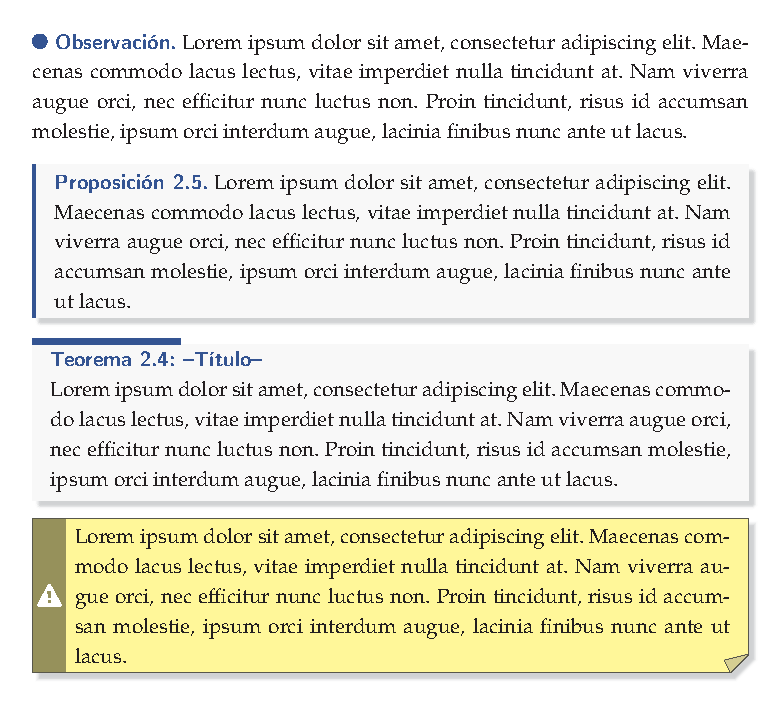
\includegraphics[scale=0.8]{Figuras/TeoNuevo.eps}
    \caption{Ejemplo ambientes de teorema}
    \label{fig:04}
\end{figure}


\section{Ejemplos}

El inicio de un libro utilizando esta clase suele tener la siguiente forma:
\begin{verbatim}
    \documentclass[10pt]{aleph-libro}

    % -- Paquetes adicionales
    \usepackage{enumitem}
    \usepackage{amssymb}

    % -- Datos del libro
    \autor[A. Merino]{Andrés Merino}
    \titulo{Matemática para diseño}
    \subtitulo[:]{Herramientas básicas}
    %\fasciculo{Número reales}
    \numero{1 (1)}
    \serie{Cuadernos de Matemática\\[1mm] Escuela de Ciencias}{Cuaderno de matemática de la Escuela de Ciencias}
    \editor{Andrés Merino}
    %\revision{}
    %\asistente{}
    \fechapub{2023}
    \edicion{Segunda}{2023}
    \impresion{Primera}{2018}
    \registroautoral{}
    \ISBN{978-0-00000-000}
    \publicado{en linea por Andrés Merino,\par Quito, Ecuador.}
    \derechos{Andrés Merino}
    \nota{Queda pro}

    % -- Logos
    \logouno{Logos/logo03}{3cm}{2.5cm}
    \logodos{Logos/logo01}{3cm}{2.5cm}
    \logofondo{Logos/logoFondo}

    % -- Colores
    \definecolor{colorp}{cmyk}{0.81,0.62,0.00,0.22}
    \definecolor{colordef}{cmyk}{0.81,0.62,0.00,0.22}

    % -- Otras adaptaciones
    \ecuadroblanco{.32\paperwidth}

    % -- Fuentes
    \fuente{montserrat}
\end{verbatim}
Con esto se obtiene las imágenes indicadas en la Figura~\ref{fig:01}.

\begin{figure}[H]
    \centering
    \fbox{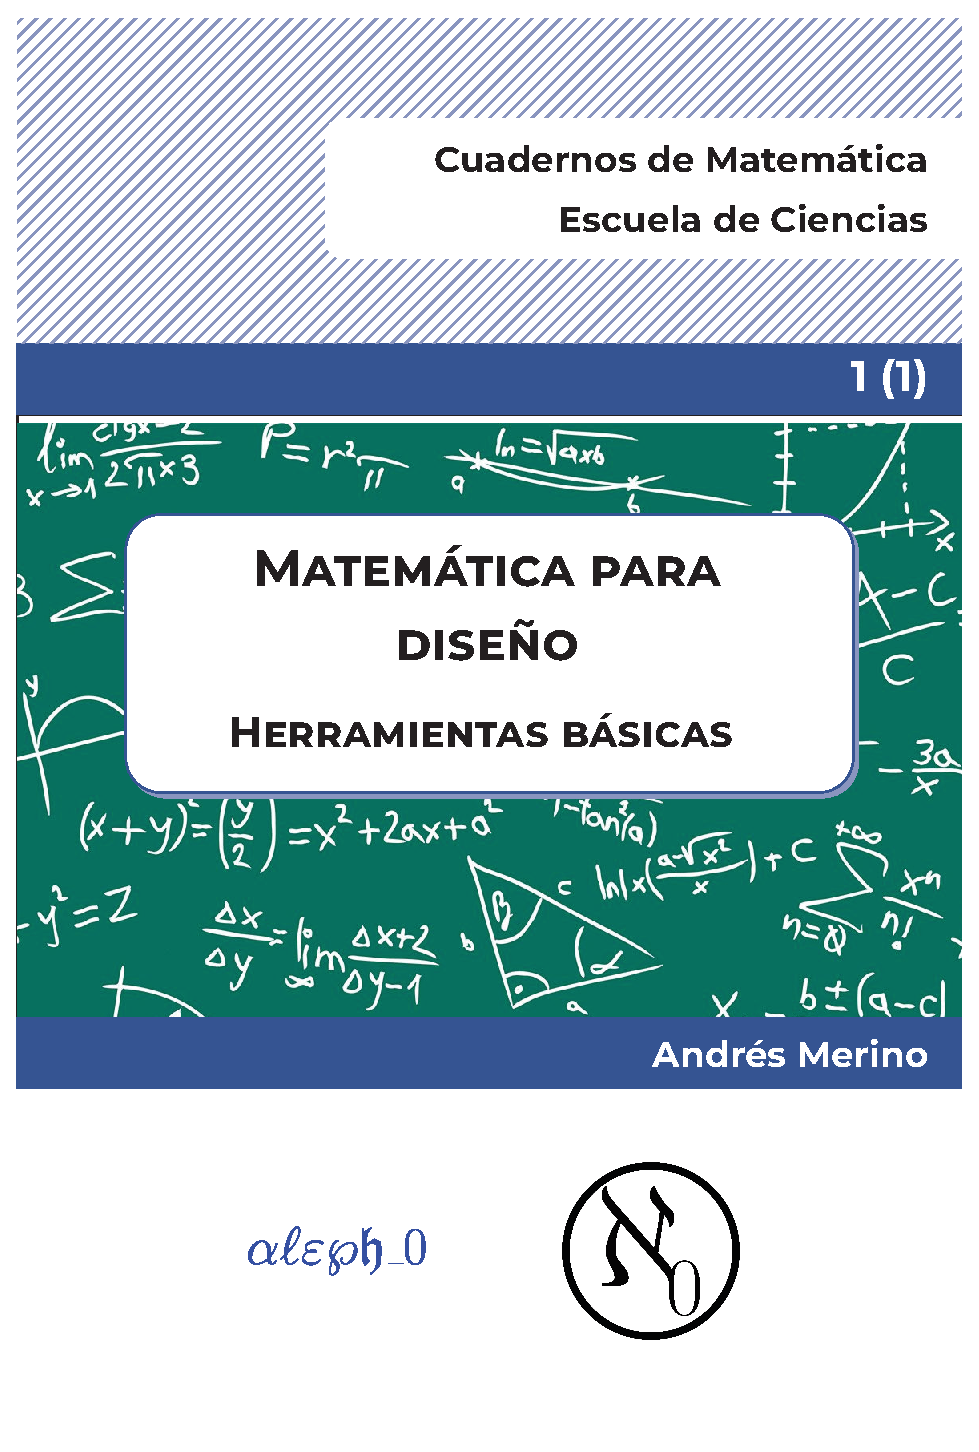
\includegraphics[scale=0.35]{Figuras/pag01.eps}}\hspace{5mm}
    \fbox{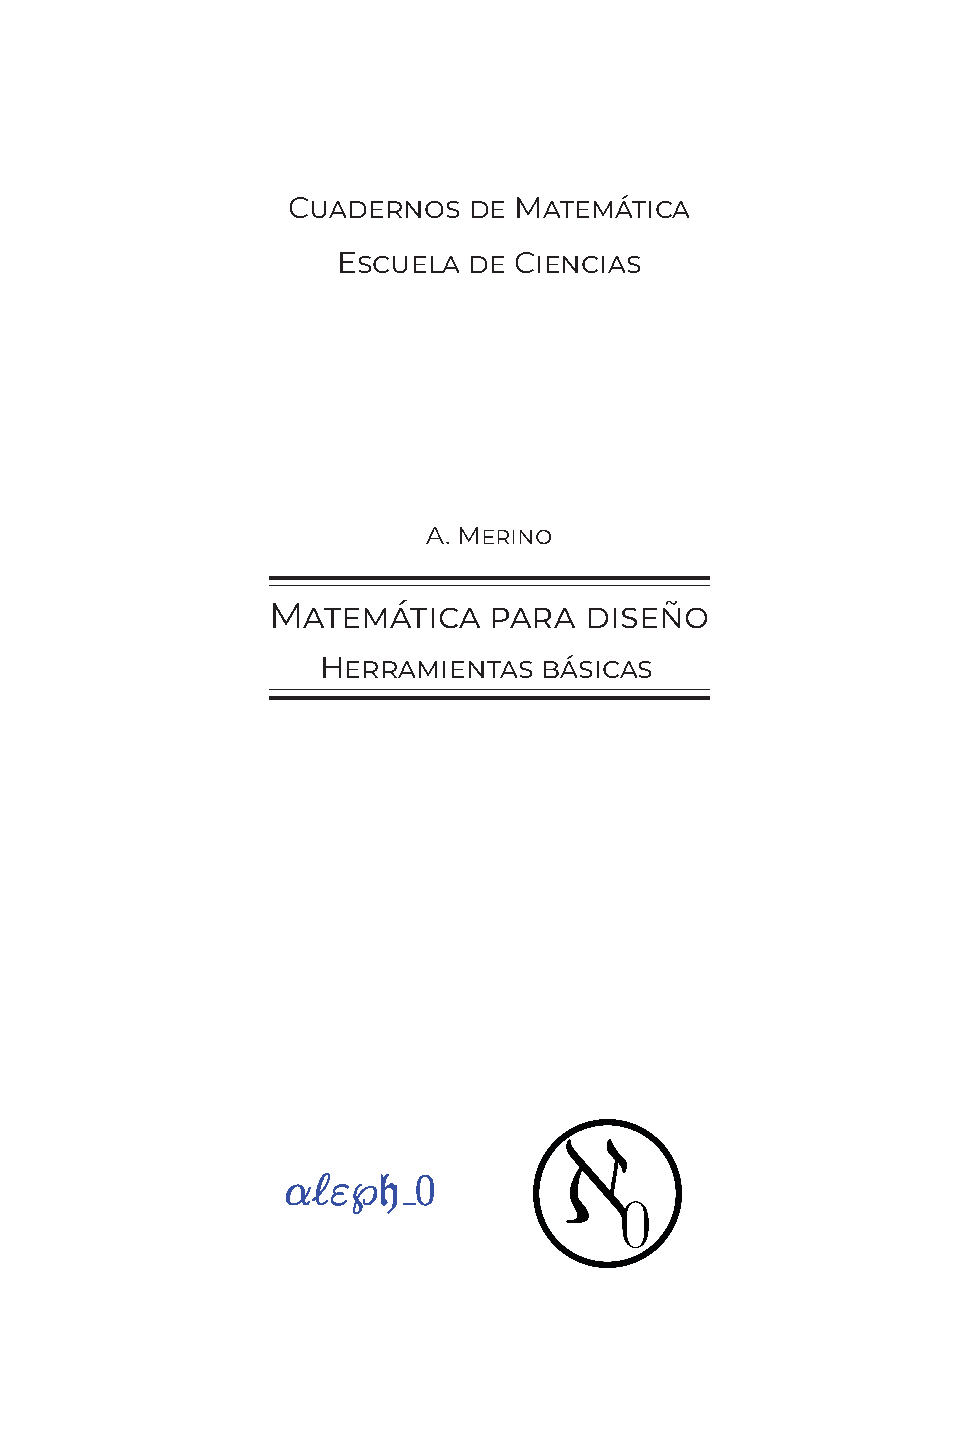
\includegraphics[scale=0.35]{Figuras/pag02.eps}}\\[5mm]
    \fbox{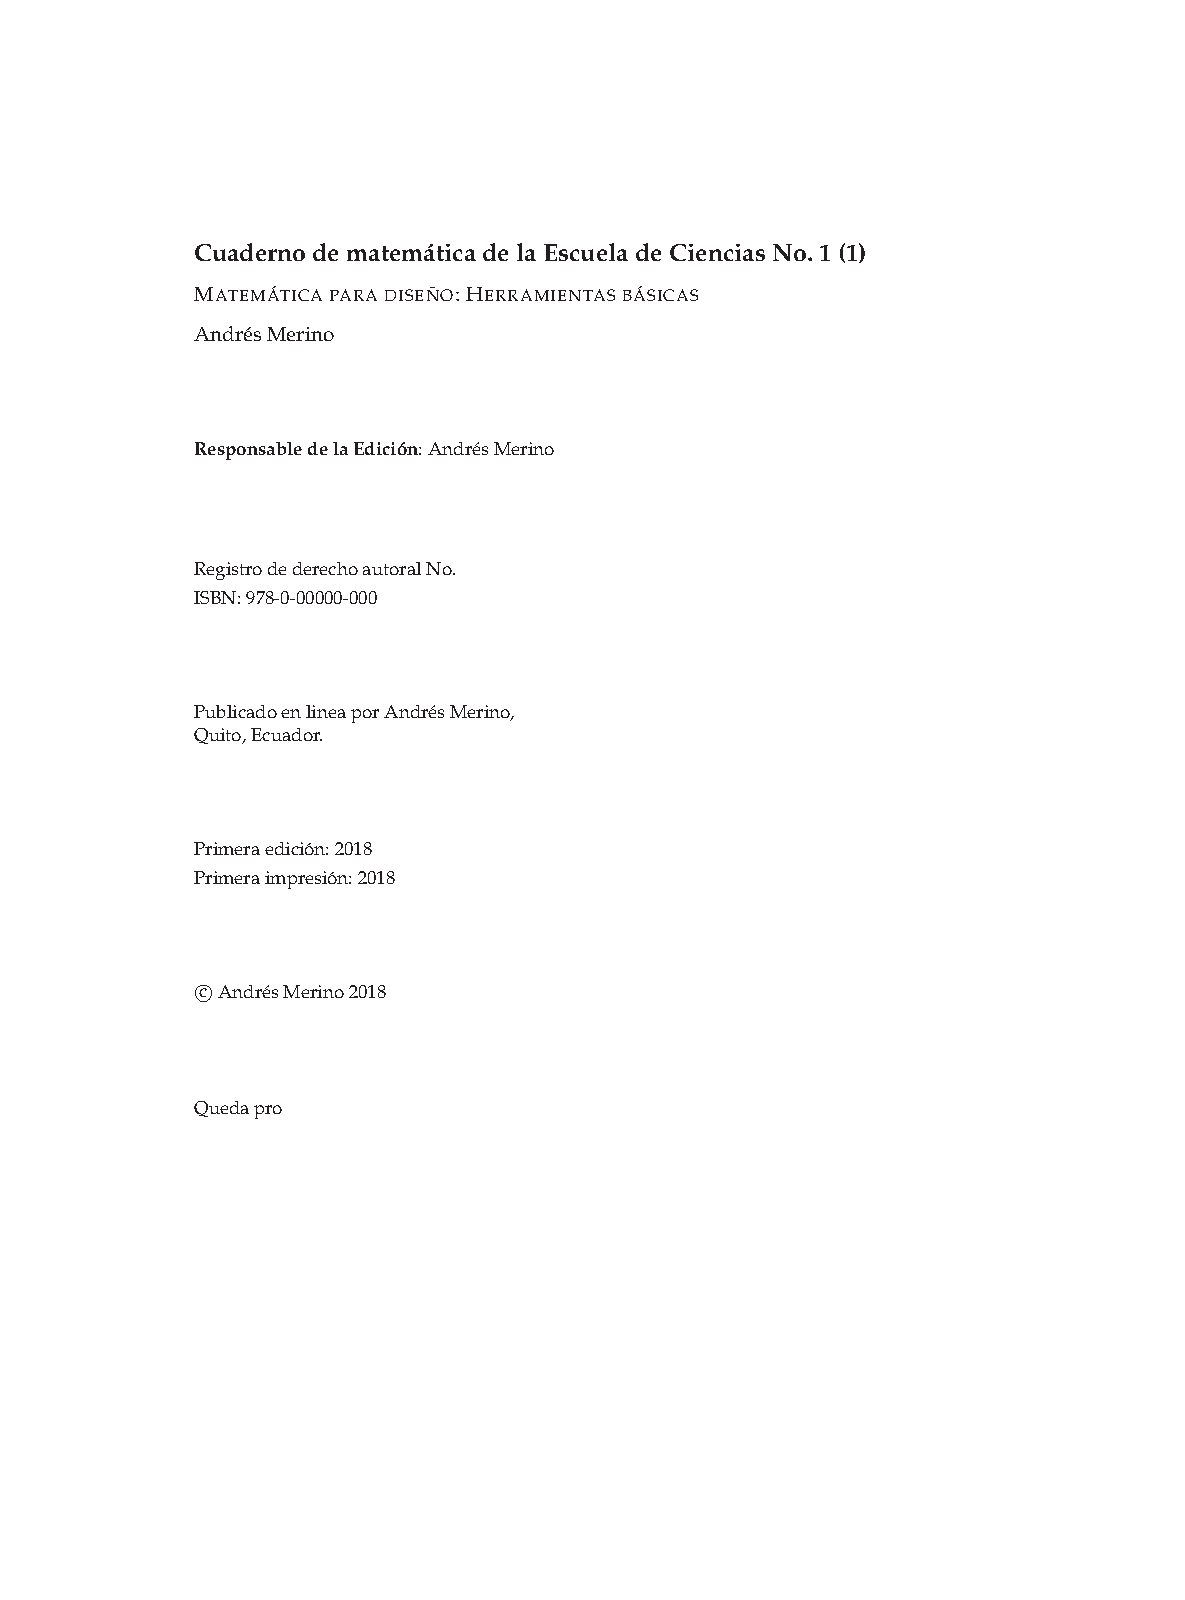
\includegraphics[scale=0.35]{Figuras/pag03.eps}}
    \caption{Ejemplo de libro}
    \label{fig:01}
\end{figure}

También se pueden generar más ambientes de teoremas, con otros formatos y colores, siguiendo los siguientes ejemplos (con título aparte, por el momento, todos los ambientes deben numerarse por capítulos y sus respectivos contadores deben ser redefinidos como se muestra). 

\begin{verbatim}    
    % - Ambientes sin recuadro
    \theoremstyle{estiloteoreman}
        \newtheorem*{pncero}{\color{red} \tikz \fill (1ex,1ex) circle (3.5pt); Personalizado cero}
    
    % - Ambientes con recuadro sin titulo aparte
    \theoremstyle{estiloteoreman}   
        \newtheorem{pnuno}[propn]{Personalizado Uno}
            \tcolorboxenvironment{pnuno}{%
                color=brown,recuadrost,colback=red!10,drop fuzzy shadow
            }
    
    % - Ambientes con título aparte con otra numeración
    \newcounter{pnumnn}[chapter]
    \renewcommand{\thepnumnn}{\thechapter.\arabic{pnumnn}}
    \newtcolorbox{pndos}[1][]
        {tipo=Personalizado Dos,contador=pnumnn,color=magenta,recuadroctint={#1}}
    
    \newtcolorbox{pntres}[1][]
        {tipo=Personalizado Tres,contador=pnumnn,color=olive,recuadroctint={#1},
        colback=lime,colbacktitle=lime,colframe=lime}
\end{verbatim}
Con esto se obtiene la imagen indicada en la Figura~\ref{fig:05}. 

\begin{figure}[H]
    \centering
    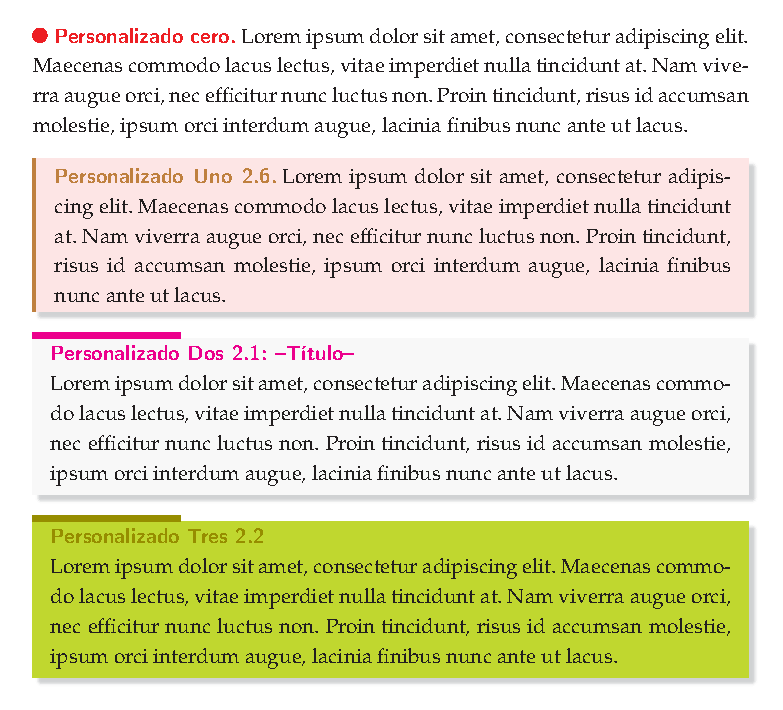
\includegraphics[scale=0.98]{Figuras/ReTeoNuevo.eps}
    \caption{Ejemplo de redefinición en estilo nuevo}
    \label{fig:05}
\end{figure}


\section{Problemas}

\begin{itemize}
\item
    Siempre que se utilicen notas al margen es obligatorio no retirar la página luego de la portada.
\item 
    La versión actual trabaja bien en la versión de TeXLive 2019 en adelante (específicamente, con el paquete \package{tcolorcox} v4.20). Si se usa una versión anterior, existe una incompatibilidad con la actualización del paquete. Para utilizar versiones anteriores de ese paquete, es necesario cambiar:
    \begin{itemize}
        \item |tcbcolback| por |tcbcol@back|
        \item |tcbcolframe| por |tcbcol@frame|
    \end{itemize}
\item
    La versión actual genera páginas en blanco antes de la portada.
\end{itemize}

Cualquier otro problema adicional, por favor reportarlo a\\ 
\url{mat.andresmerino@gmail.com}.

\begin{changelog}[author=Andés Merino,
    sectioncmd=\section]
    % version 2.0
    \begin{version}[author=Daniel Lara,v=2.0,
        date=2023-12-24]
        \removed
        \item Se elimina el formato clásico para el estilo de los teoremas.
        \added 
        \item Se añade la posibilidad de seleccionar fuentes: Palatino Linotype (Mathpazo) y Monstserrat
        \fixed 
        \item Se ha optimizado la generación de recuadros utilizando el paquete |tcolorbox|.
    \end{version}
    % version 1.1
    \begin{version}[v=1.2.1,
    date=2020-08-14]
    \added
    \item Se incluye estilos de formato para ambientes: fclasico, fnuevo
    \end{version}
    % version 1.0
    \shortversion{v=1.2,
    date=2020-01-07,
    changes=Primera versión del paquete \texttt{aleph-libro}}
    % version 0.1
    \shortversion{v=0.1,
    date=2019-05-05,
    changes=Última versión del parquete \texttt{pubciencias-notas}}
\end{changelog}

\newpage
\DocInput{aleph-libro.dtx}

\end{document}